\documentclass[12pt]{article}
\usepackage[english]{babel}
\usepackage{t1enc}
\usepackage{bm}

% AMS packages:
\usepackage{amsbsy}
\usepackage{amsfonts}
\usepackage{amsmath}
\usepackage{amssymb}
\usepackage{amsthm}
\usepackage{amsxtra}
% for comments to work
\usepackage{verbatim}
\usepackage{hyperref}
\usepackage{graphics}
\usepackage{graphicx}
%%for typing code
%\usepackage{listings}
%%for breaking lines when typing code
%\lstset{breaklines=true}
%%Matrix syntax
\usepackage{tikz-feynman}






% $$\left(\begin{array}{rrrr}
	%	1-\kappa -\gamma_1& -\gamma_2 \\
	%	-\gamma_2 & 1-\kappa -\gamma_1 \\
	%\end{array}\right)$$
	
	
%%System of equations syntas

% \begin{cases}
	%	\frac{1}{1-\frac{r_s}{r}} \left(\frac{dr}{d r'}\right)^2 = B(r')\\
	%	r^2 = B(r') {r'}^2
	%\end{cases}
	
	
	%%Fit formula to size
	
	%$$\resizebox{\linewidth}{!}{$  FORMULA
		%	$}$$
	
	%\title{T\'itulo}
	%\author{}
	%\date{\today}
	
\begin{document}
	%	\maketitle

\begin{figure}[h]
\centering
	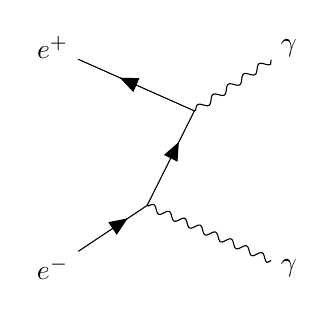
\begin{tikzpicture}
		\begin{feynman}
			\vertex (a) {\(e^{+}\)};
			\vertex [right=1.2of a] (a1);
	    	\vertex [right=1.8of a] (a2);
			\vertex [below =0.8of a2] (b);
			\vertex [right=3of a] (f1) {\(\gamma\)};
			\vertex [below =2of  a1] (c);
			\vertex [below =2.8of f1] (f2) {\(\gamma\)};
			\vertex [below =2.8of a] (f3) {\(e^-\)};
			
			\diagram* {
				(a) -- [anti fermion] (b) -- [boson] (f1),
				(b) -- [anti fermion] (c),
				(c) -- [boson] (f2),
				(c) -- [anti fermion] (f3),
			};
		\end{feynman}
	\end{tikzpicture}\quad\quad
	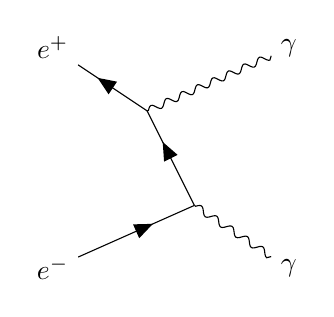
\begin{tikzpicture}
		\begin{feynman}
		\vertex (a) {\(e^{+}\)};
		\vertex [right=1.2of a] (a1);
		\vertex [right=1.8of a] (a2);
		\vertex [below =0.8of a1] (b);
		\vertex [right=3of a] (f1) {\(\gamma\)};
		\vertex [below =2of  a2] (c);
		\vertex [below =2.8of f1] (f2) {\(\gamma\)};
		\vertex [below =2.8of a] (f3) {\(e^-\)};
		
			\diagram* {
		(a) -- [anti fermion] (b) -- [boson] (f1),
		(b) -- [anti fermion] (c),
		(c) -- [boson] (f2),
		(c) -- [anti fermion] (f3),
	};
	   \end{feynman}
	\end{tikzpicture}
    \caption{Feynman graphs for the lowest order contributions to electron annihilation [\ref{Martin}].}

\end{figure}

\begin{thebibliography}{10}	
	
	\bibitem{Martin}\label{Martin}
	B. Martin ang G. Shaw,
	\textit{John Wiley \& and sons, 1992.}
\end{thebibliography}
\end{document}
